\chapter{RFP Equilibrium}
\label{section:2_equilibrium}

The success of electromagnetic containment systems depends on the ability to maintain the plasma in equilibrium in the presence of small perturbations
that could compromise its stability. In Tokamak and RFP type experiments, the instabilities that produce macroscopic effects are described, in their simplest form, by the plasma fluid model MHD ( magnetohydrodynamic model ). 
We abandon the kinetic description of the single particle to consider the set of charges, thinking of the plasma as a fluid: the dimensions of the survey region are much greater than the Debye length and the Larmor radius. Therefore, a discrete system with separate charges is no longer observed.


%  __  __ _   _ ____  
% |  \/  | | | |  _ \ 
% | |\/| | |_| | | | |
% | |  | |  _  | |_| |
% |_|  |_|_| |_|____/ 


\section{Single fluid magnetohydrodynamic equilibrium}

In the MHD model the equations of classical electromagnetism are combined with those of the fluid motion. Typically the analysis of fluid plasma involves the generalized movements of each ionic species; however, for simplicity it is possible to consider each pair of values relating to ions and electrons in a single parameter and thus obtain a single fluid trend. Moreover, remembering that for fusion gases there is almost neutral charge $n_i = n_e$ the charge density term $\rho = e(n_i - n_e)$ can be omitted. The relevant quantities are thus:
\begin{itemize}
    \item the mass density of the fluid
    \begin{equation}
        \rho_m = n_e m_e + n_i m_i
    \end{equation}
    \item the mean current density per unit volume
    \begin{equation}
        \mean{J} = e(n_i \mean{v_i} - n_e \mean{v_e})
    \end{equation}
    \item the fluid pressure
    \begin{equation}
        p \approx n_e k T_e + n_i k T_i
    \end{equation}
\end{itemize}
With this variables the fluid equations and the conservation of moment and mass can be defined:
\begin{align}
    \pdv{\rho_m}{t} + \nabla \cdot (\rho_m \Vec{v}) &= 0 \\
    \rho_m \left( \pdv{\Vec{v}}{t} + \Vec{v} \cdot \nabla \Vec{v} \right) &= \Vec{J} \times \Vec{B} - \nabla p
    \label{eq:mhd_momentum} 
 \end{align}
where the electromagnetic interaction can be added with the Maxwell and Ohm relations:
\begin{align}
    \nabla \times \Vec{E} &= - \pdv{\Vec{B}}{t} \label{eq:faraday} \\
    \nabla \times \Vec{B} &= \mu_0 \Vec{J} \label{eq:ampere} \\
    \nabla \cdot \Vec{B}  &= 0 \\
    \nabla \cdot \Vec{E}  &= 0 \\
    \Vec{E} + \Vec{v} \times \Vec{B} &= \eta \Vec{J} \label{eq:ohm}
\end{align}
Finally to close the system you can choose to introduce alternatively:
\begin{itemize}
    \item the perfect conductivity of the plasma to obtain the cancellation of the resistivity\footnote{In fact the resistivity is a term related to the plasma temperature through the Spitzer relation \begin{equation}
        \eta = 5 \times 10^{-5} \frac{Z \log(\Delta)}{T_e^{3/2}}
    \end{equation}} term in \eqref{eq:ohm}
    \begin{equation}
        \eta = 0
    \end{equation}
    \item teh addition of a state constraint for the ideal gas, considering only isothermal or adiabatic transformations:
    \begin{equation}
        \pdv{}{t}\left( \frac{p}{\rho_m^\gamma} \right) = 0
    \end{equation}
    \begin{align}
        \gamma &= 1    \hspace{3cm} & \text{isotherms} \\
        \gamma &= 5/3  \hspace{3cm} & \text{adiabatic}
    \end{align}
\end{itemize}
From the MHD equations it is also possible to derive some considerations regarding the movement of the plasma: for example, combining the Ampere equation \ref{eq:ampere} with that of Ohm \ref{eq:ohm} we obtain the variation of the induction field, which turns out to be the composition of a flow term and a field diffusion term.
\begin{equation}
    \pdv{\Vec{B}}{t} = \nabla \times ( \Vec{v} \times \Vec{B} ) + \frac{\eta}{\mu_0} \nabla^2 \Vec{B}
    \label{eq:coupling_plasma_1}
\end{equation}
This report describes the dynamic coupling between the magnetic field and the displacement of the fluid. If we compare the two contributions of \eqref{eq:coupling_plasma_1}, considering as viscosity factor $\nu_m = \eta/\mu_0$, we get:
\begin{equation}
    \frac{|\nabla \times \Vec{v} \times \Vec{B}|}{|\nu_m \nabla^2 \Vec{B}|} \simeq \frac{\frac{x \cdot B}{L}}{\nu_m\frac{B}{L^2}} = \frac{vL}{\nu_m} \equiv \mathcal{R}_m
\end{equation}
where L is the characteristic variation length for the quantities considered. $R_m$ is called Magnetic Raynolds Number and quantifies the prevalence of plasma flow phenomena with respect to $\Vec{B}$ diffusion.

When, as generally happens, it is the first component to be dominant $(R_m >> 1)$, the relationship expresses the conservation of the magnetic flux through any surface bounded by a closed line, independently of the movement of the fluid. This result is also expressed by Alfven's theorem: in a conductive fluid with zero (or very small) resistivity, the magnetic field lines remain frozen in a given volume of the fluid itself.
In conclusion it can be said that a plasma of small magnetic viscosity can be more effectively compressed by strong gradients; at the same time, however, a turbulent motion is obtained in which the variation of the field increasingly depends on transport phenomena.




\subsection{Static equilibrium}
The study of the plasma MHD instability mainly concerns the perturbations of the ideal system starting from a magneto-static equilibrium point. In this state the relationships that present a temporal variation are null, thus, imposing $\eta=0$ and $\pdv{}{t} = 0$ the system become:
\begin{align}
    & \nabla \cdot \Vec{B} = 0 \\
    & \nabla \times \Vec{B} = \mu_0 \Vec{J} \\
    & -\nabla p + \Vec{J} \times \Vec{B} = 0
\end{align}
% \begin{equation}
% \systeme*{
%     \nabla \cdot \Vec{B} = 0,
%     \nabla \times \Vec{B} = \mu_0 \Vec{J},
%     -\nabla p + \Vec{J} \times \Vec{B} = 0
% }
% \end{equation}
From the third equation it is clear that the pressure gradient is maintained orthogonal to the field and current lines, constructing a set of surfaces, one inside the other~(\Figure{}), called toroidal isobar magnetic surfaces\footnote{It should be noted that the magnetic and current fields of the first and second relations are solenoidal and lead to necessarily closed surfaces. If we consider a constant pressure module along this surface, with an intersection angle between the perpendicular field vectors everywhere, we obtain the torus as a possible solution.}. These are said rational surfaces when the field lines that run through them recombine on themselves after a few toroidal turns, or ergodic when, not recombining, they cover the entire surface.

The effects of a generic stability disturbance of the balance just described is now explicitated using the spatial transformation in Fourer series; the perturbation $\Tilde{\psi}$ can be expressed as:
\begin{equation}
    \Tilde{\psi}(\Vec{r},t) = \sum_k \Tilde{\psi}_k(r) e^{i(\Vec{k}\cdot\Vec{r}-\omega t)} = \sum_k \Tilde{\psi}_k e^{i(m\vartheta+n\varphi-\omega t)}
\end{equation}
where $\Vec{r} = (r,\vartheta,\varphi)$ is the displacement vector in toroidal coordinates, and $\Vec{k}$ is the vector of the respective wave numbers.

Its frequency is the expression of the transform in time, and it is in general a complex value $\omega = \omega_R + i \omega_I$, in which the real part expresses the propagation speed of the wave, and the imaginary part represents the growth, damped $(\omega_I < 0)$ or exponential $(\omega_I > 0)$, of the amplitude of the perturbation. The step of this perturbation is therefore obtained by $(m\vartheta + n\varphi = \text{const})$, that is:
$$  m d\vartheta - n d\varphi = 0    $$
$$  p_p = \int_0^{\Delta\varphi} d\varphi = \int_0^{2\pi} \frac{m}{n}d\vartheta = \frac{m}{n} 2\pi  $$
In the same way the step for the field lines is:
$$  \frac{R_0 d\varphi}{r d\vartheta} = \frac{B_\varphi}{B_\vartheta} $$
$$  p_b(r) = R_0\Delta\varphi = \int_0^{2\pi} \frac{1}{R_0} \frac{B_\varphi(r)}{B_\vartheta(r)} r d\vartheta = 2\pi r \frac{B_\varphi(r)}{B_\vartheta(r)}  $$

\begin{equation}
    p_b(r) = p_p    \hspace{2cm} 	\iff \hspace{2cm}  q(r)\equiv \frac{r}{R_0}\frac{B_\varphi(r)}{B_\vartheta(r)}=\frac{m}{n}
\end{equation}



The perturbation $\tilde{\psi}(m,n)$ whose steps are coupled with the field lines is called \textit{resonant}, and is the cause of instability. In this picture it is evident that the \emph{'' safety factor ''} $q(r)$ is related to the stability of the plasma; in fact, if $q$ is rational, any displacement of the plasma from the equilibrium position can have a component that is screwed onto the magnetic surfaces with the same periodicity as the field. If, on the other hand, $q(r)$ is irrational the field lines continue to be screwed onto the toroidal surface without ever rejoining with themselves, sweeping ergodically the entire surface.


%%%%%%%%%%%%%%%%%%%%%%%%%%%%%FIGURA%%%%%%%%%%%%%%%%%%%%%%%%%%%%%%%%%%%%%
\begin{figure}[ht!]
 \centering
 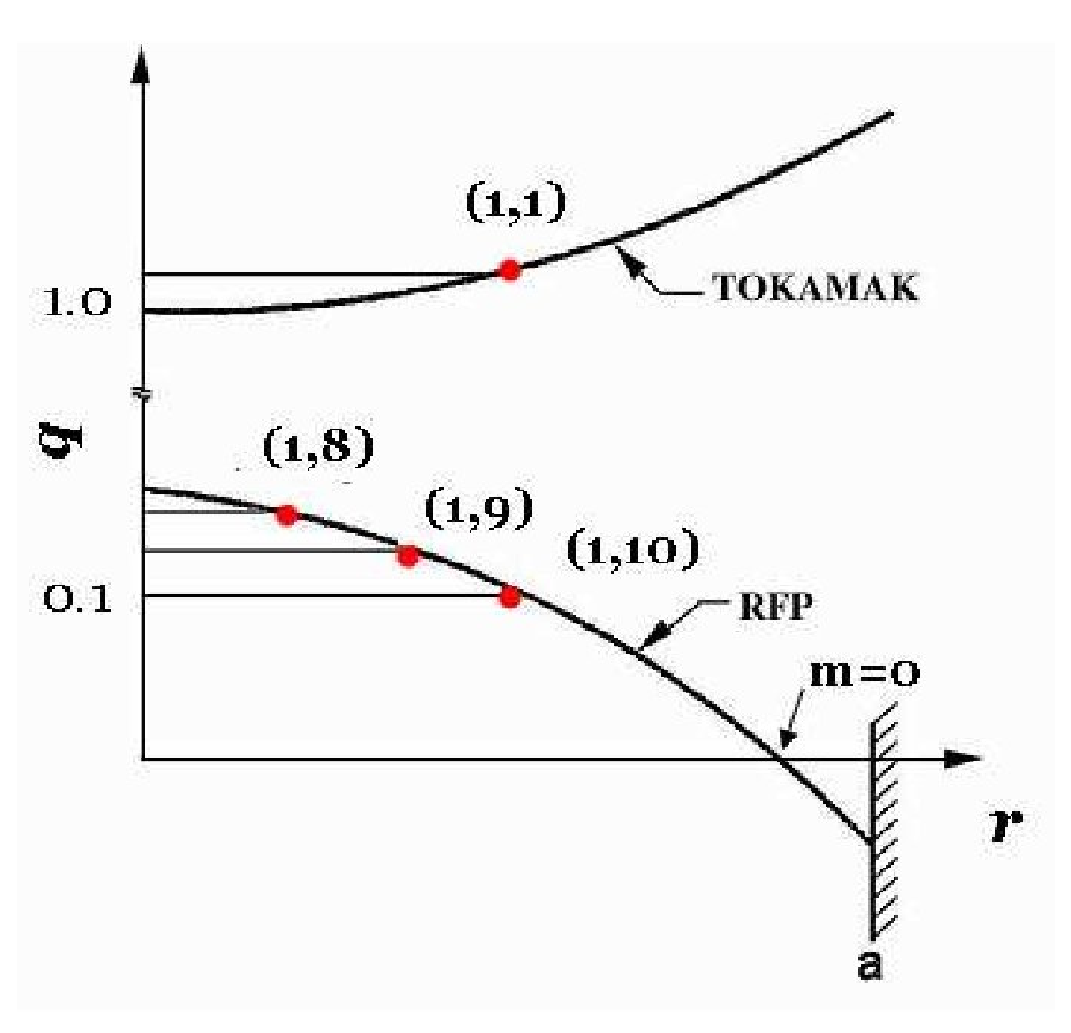
\includegraphics[ width=8cm ] {img/2_eq/safety-tokarfp.eps}
 \caption{Comparison of $q$ profiles, with respect to the position of the torus axis; for Tokamak and RFP type machines. }
 \label{fig:profiles-tokarfp}
\end{figure}
%%%%%%%%%%%%%%%%%%%%%%%%%%%%%%%%%%%%%%%%%%%%%%%%%%%%%%%%%%%%%%%%%%%%%%

In turn, more adjacent surfaces that have the same safety factor couple with each other giving rise to resonance phenomena, becoming themselves a source of instability; for this reason we introduce the parameter called the \emph{'' shear ''}
%
\begin{equation}
 s(r) \equiv \frac{r}{q(r)}\frac{dq(r)}{dr} = \frac{r}{p_b}\frac{dp_b}{dr}
\end{equation}
%
it represents the variation along $r$ of the pitch of the field lines. It is therefore essential that the pitch is variable monotonically to avoid destabilizing the entire system.
In \Figure{\ref{fig:profiles-tokarfp}} the radial profiles of the safety factor for Tokamak and RFP experiments are plotted; note that the configuration has been chosen in such a way that the trends represent strictly monotone functions.

\subsubsection{The cylindrical approximation}

Although the real machine has a toroidal shape, to simplify the treatment of the forces involved in the MHD model it is considered a cylindrical approximation, ideally imposing also the quantities along the longitudinal axis of the cylinder periodic. In this particular geometry, which will also be used for the study model subject of the present discussion, it is easier to identify the two current configurations that realize the  \emph{''pinch''} effect (striction) of the plasma \cite{fridberg}\cite{ortolani}, called $theta$-\emph{pinch} and $zeta$-\emph{pinch}\footnote{currents along the angular and axial direction of the cylinder, transformations of the poloidal and toroidal coordinates respectively.}.

For example, inserting the Ampere equation \eqref{eq:ampere} into the Navier-Stokes \eqref{eq:mhd_momentum} of the continuity of the momentum, we obtain a relation that describes the behavior of the pressure in the plasma:
\begin{equation}
 \label{eq:mhd_sol1}
 -\nabla \left( p+\frac{B^2}{2\mu_0} \right) + \frac{
  (\Vec{B}\cdot\nabla)B}{\mu_0} = 0
\end{equation}
Still remaining in the steady state of equilibrium, where the term of time derivative is null, the \eqref{eq:mhd_sol1} describes the equilibrium that is established between the pressures, kinetic and magnetic, and the effect of the curvature of the ${B}$ field lines (so-called magnetic tension). If we consider, then, a simple example of linear pinch, in which the magnetic tension component also disappears, the magnetic tension is in fact an expression of the curvature of the field lines, we can see how the striction effect depends on the gradient of field of the plasma column. Thus it is possible to reformulate the parameter $ \beta $ which for the linear pinch depends precisely on the relationship between the external field and the field penetrated into the plasma:
\begin{equation}
\beta = \frac{p}{p_{mag}} = 1-\frac{B_{int}}{B_{ext}}
\end{equation}



\subsection{Classification of instabilities}
\label{sez:classificazione}

The general classification of plasma instabilities is usually based either by their main physical causes, or the place where they rise up.
%
In the former case we divide them by the source of destabilization, there can be instabilities: pressure driven, current driven or particle driven. 
The pressure driven modes, also called “pressure driven instabilities” ( for example “interchaged modes or balooning modes” are pressure driven), can be derived directly from the equilibrium equation (force balance between kinetic and magnetic pressure) when we have strong gradient in the perpendicular current.
The current driven modes are instabilities that grow in time, they dissipate energy. In this case the parallel current gradient is the main driving phoenomena: kink modes are an example of current driven instabilities. Kink modes can be either internal or external; and usually the external kink sets the actual limit on the maximum achievable current. So the q factor at the edge instability is set by an external kink. Certainly they can also combine and give rise to a balooning-kink mode.

In the second class we divide instabilities based on the place where they rise; they can be: external (edge boundary involved) or internal (only inside plasma) modes. 
They are also called \emph{fixed-boundary} and \emph{free boundary} instabilities when identified with respect to the column surface displacement. The former have an effect inside the column, not affecting the movements of the plasma surface, the latter \emph{free boundary} instabilities are macroscopic and involve the overall displacement of the vacuum-plasma interface.
This is the worst case because in this way the overall confinement is usually lost: if such an instability development the plasma changes shape and could touch directly the first wall and the first facing components. This is dangerous because you have a parallel flux of energetic particles going directly to the materials, and a strong plasma wall interaction pollutes the gas leading to the end of the discharge.
%
Any mode can be further subdivided based on the wave numbers that describe the relative perturbation $\tilde{\psi}(\Vec{r}) =
\Tilde{\psi}_0(r)e^{i(m\vartheta+n\varphi)}$.
%
The poloidal modes\footnote{generally the perturbation is expressed with the term way to indicate the pair of values $(m, n)$} of number $m = 0$ give rise to instability called \emph{`` sausage instabilities ''}, and are due to flow exchanges. These instabilities can be easily described by observing a pure z-\textit{pinch} experiment in cylindrical geometry: as shown in the \Figure{\ref{fig:press-curr1}}, the axial constrictions of the plasma column involve different values of $B_\theta \sim 1/r$. The kinetic pressure is the same everywhere, while the magnetic pressure tends to be stronger at the saddle, giving rise to bulges that are increasingly amplified.
%
\begin{figure}[ht]
 \centering
 \subfigure[]{ \label{fig:press-curr1}
 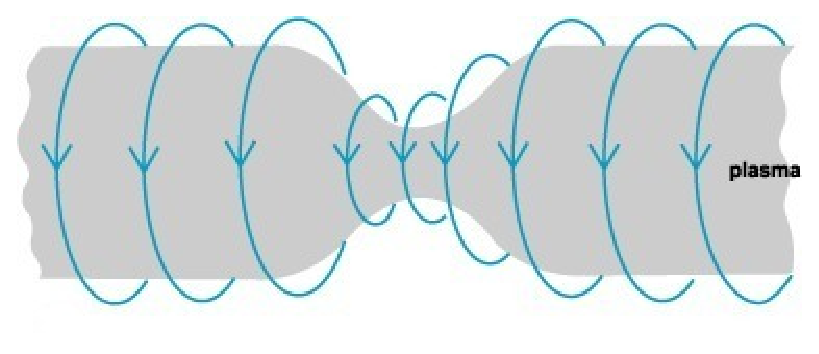
\includegraphics[ width=5cm ] {img/2_eq/press-curr1.eps}}
 \subfigure[]{ \label{fig:press-curr2}
 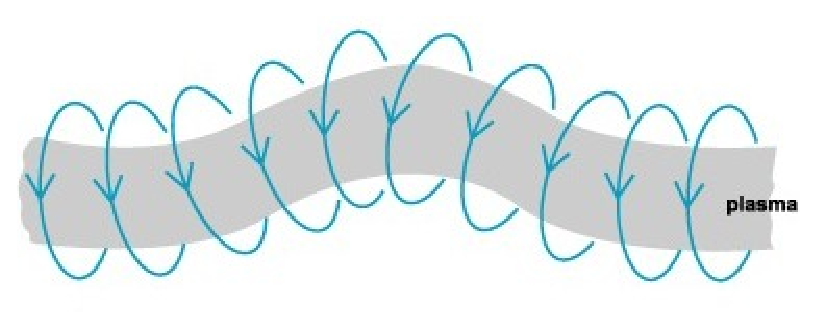
\includegraphics[ width=5cm ] {img/2_eq/press-curr2.eps}}
 \caption{Pressure and current instabilities}
\end{figure}
%
The modes of poloidal number $m = 1$ give rise, instead, to instabilities called \emph{``kink instabilities''}, \Figure{\ref{fig:press-curr2}}. In this case the curvature of the column of plasma involves the thickening of the field at the lower surface concave part; there is again an increase in the magnetic pressure which gradually tends to amplify itself.
%
These instabilities are quite dangerous, as they are often rapid and so it is hard to get rid of them, with growth times in the order of $1/\tau_A$ \footnote{$\tau_A = a/v_A$, with $ v_A $ the Alfvén speed and $a$ the minor torus radius, it refers to field variations frozen plasma \cite{fridberg}.}; they are mainly built in the presence of resonant surfaces and are generally stabilized by a strong toroidal field.

As a conclusion of the considerations made in the previous paragraph regarding the safety factor $ q $ and the shear, it is interesting to mention now the the Kruskal-Shafranov criterion for stability in Tokamak configurations. In modes $ m = 1 $ we have resonance for $q(r)=1/n$; to ensure stability it is necessary to keep $ q>1 $. However it is important to remember that $ q (r) $ has a minimum trend in the center of the column and increases towards the periphery; therefore, because the criterion holds everywhere, it is good that the value of $ q $ on the periphery remains bounded as $ 2<q(a)<3 $\footnote{therefore, on the basis of these observations, placing the value at the periphery of $q(a)=\frac{a}{R_0}\frac{B_\varphi(a)}{B_\vartheta(a)}~\simeq~3$ and considering an aspect ratio $a/R_0 \simeq 3$, we explain the presence of a strong imbalance between the fields $B_\varphi$ and $B_\vartheta$ in the Tokamak configuration.}.


\subsection{The resistive wall modes}

An important example of \textit{kink instability} is represented by the so called \ac{RWM}. They are formed by the non zero resistance of the conductive shell; they are relatively slow since they depend on the time of penetration of the field into the material of the shell $\gamma_{RWM} \propto 1/\tau_w$. Their value is defined as:
%
\begin{equation}
 \tau_w = \mu_0 \sigma r_w \delta_w
\end{equation}
%
where $\sigma$ is the conductivity of the wall, $ r_w $ the corresponding radius and $\delta_w \ll r_w$ the wall thickness. The \acs{RWM}s are characterized by the presence of a radial field $b_r|_{r=r_s} \neq 0$, where $ r_s $ is the radius of the resonant surface that generates the unstable mode, which makes the recombination of the field lines possible.
%
A spontaneous growth of \acs{RWM} instability has been experimentally observed in \acs{RFP} with non-resonant \emph{'' current driven ''} perturbations characterized by $ m = 1 $, and several harmonics $ n $ which can be simultaneously unstable with different growth factors $\gamma$\cite{pizz46}\cite{pizz47}\cite{gregoratto}.

In Tokamak configurations the spectrum of RWM modes is usually characterized by the dominant toroidal component of mode $ n = 1 $ and by various poloidal modal components with $m=2,3,4$ etc.\footnote{
However, recent experiments shown that in some Tokamak configurations there is the presence of ideal \textit{kink} instabilities of non-resonant \emph{current driven} modes. These instabilities seem to be excited by the free energy in the gradients of the plasma current that arise during the ascent current ramp~\cite{baruzzo9, baruzzo10, baruzzo11}. This effect has the double disadvantage of limiting the maximum growth rate obtainable for the induction of the plasma current and, at the same time, they define a minimum value of the safety factor at the edge.}.
%
Usually the study of \acs{RWM}s is conducted in \acs{RFP} configuration, because in this context they are more easily reproducible and do not cause great damage to the walls of the chamber. Nevertheless, their stabilization is an important challenge also for modern Tokamak machines, being one of the main factors that limit the high $\beta$ configurations.

To control the wall modes, in recent years some stabilization methods applicable to both the two configurations have been studied. Among these the stabilization based on the plasma rotation effect consists in the production of a toroidal angular momentum through the orientation of the neutral beam injector. This theory suggests that stabilization can be effectively achieved for angular velocities above a critical value ($\Omega_c \thickapprox 1KHz$) However, experimental observations have shown that, although this value is sufficient to maintain stability, in fact it is not compatible with values of $\beta$ above a certain threshold \cite{baruzzo12}. In fact, beyond a given restriction, the plasma tends to slow down the rotation, creating the conditions for the onset of \acs{RWM}. This method is effective for ensuring the functioning of recent Tokamak configurations~\cite{baruzzo12}, but not for the acs{RFP} configuration~\cite{baruzzo13}; it is also not yet clear whether it can be successfully used in the ITER project\footnote{International Thermonuclear Experimental Reactor, in Latin `` the way '': it is the machine that represents the passage between the studies performed so far on the physical and technological aspects of the fusion and the future power plant for the production of fusion energy.} due to the limited torque actually applicable by high-energy \acs{NBI}.
%
So, the solution offered by the presence of the conductive shell in the ideal wall hypothesis (perfectly conductive and continuous) has proved to be able to maintain stable equilibrium in presence of high growth factor MHD perturbations~\cite{gimblett_5,gimblett_6}; in the real case where the wall has a minimal - but not null - resistivity, the system generates \acs{RWM} type instabilities.

As already anticipated, the RFX experiment was modified with the introduction, among other innovations, of a sophisticated system of active control of the MHD modes. It consists of 192 \textit{saddle coils}: 48 poloidal arrays with 4 coils each, separately fed and located on the outer surface of the shell at a distance of $r_c = 0.5815m$. The corresponding magnetic sensors, capable of detecting the radial and toroidal field, are positioned inside the conductive wall at a distance of $r_s = 0.508m$. The control aims to counterbalance the radial field components generated by the unstable perturbations of the RWM modes. Indeed, the amplifier system is able to generate non-axisymmetric modes and can operate configured in different ways: for example the so called \emph{'' Virtual Shell ''} (VS) is a local feedback system that, while not taking account of the global effects on the plasma, is already able to strongly reduce the radial field component $b_r$\cite{pizz78}\cite{pizz79}. Other methods has been studied as well. Some propose the description of the wall crossing analyzing the aliasing components introduced by the actuators in the higher harmonics\cite{pizz81}.

%% RFP
% - Taylor relaxed state (need of reversal) -> magnetic shear
% - reversal can not be produced by coils ... plasma is needed
% - no need for superconducting coils and no current limit  -we don't satisfy Kruskal-Shafranov (safety factor)-
%   (10MA target to have a good condition in terms of neutrons production) -> ohmic heating is possible.
% - In RFX-mod the ohmic heating power can scale up to 60MW of coupled power (that is a huge amount of power)
%   in a stellarator to reach the same power deposition using external heating you need very high power.
% - High current possibility means -> High particle density limit ... Greenwald limit

% - why High plasma current? because 


\subsection{RFP Dynamo effect}

Ideal MHD means that plasma resistivity is mathematically equal to zero: this has the key direct consequence that the Alfven theorem holds. This states that the magnetic flux can be seen as ``\textit{frozen}'' inside the plasma (or in the other way around the plasma is frozen with the magnetic field line).
But in a real case scenario the plasma resistivity normally inversely depends on the temperature. The more we approach the ideal MHD conditions the more the temperature increases. The direct consequence of the ideal conditions on plasma structure topology is that it does not change maintaining closed flux surfaces; on the other hand, if plasma is thought to be resistive, there can be finite currents that dissipate energy and the topology is allowed to change yielding field lines or flux surfaces that can be cut and reconnected together. This is called \textit{magnetic reconnection}. The regions where the currents can flow are called the current sheets while the reconnected flux regions are the \textit{magnetic islands}. The plasma changes in its defined topology, and it is usually undesirable because within the magnetic islands the quality of confinement is decreased; however in certain conditions this is a good outcome for RFP as it will be shown in few lines.

What has been shown so far is that, even if in the ideal condition the plasma has been made stable through a opportunely shaped safety profile, other instabilities can rise though: due to resistive components in the MHD equation the field lines tear and reconnect each other in the so called \textit{magnetic islands}.
In an RFP system, where plasma resistivity is not null, there is a need for a mechanism to maintain the magnetic configuration balance over time otherwise diffusivity would flatten the toroidal magnetic field, the magnetic energy would be dissipated out, and the RFP configuration would be lost.
If we approximate the plasma column to a cylindrical conductor using equations given in~\eqref{eq:mhd_sol1} the magnetic field in such a condition is subject to a resistive diffusion phenomenon described by:
\begin{equation}
    \pdv{\Vec{B}}{t} = \frac{\eta}{\mu_0} \nabla^2 \Vec{B}
\end{equation}
Resolving the differential equation this field component - that describes the equivalent toroidal component in RFP - presents a decay time constant of $$\tau_R = \mu_0 a^2 / \eta$$, where $\eta$ being the resistivity of the equivalent conductor and $a$ the radius.
On the contrary the experience shows that the RFP configuration is maintained for times longer than $\tau_R$. This seems to be the result of a spontaneous mechanism of regeneration of the dissipated magnetic toroidal flow, called \textit{dynamo} in analogy with similar phenomena in astrophysical and geophysical plasmas. The dynamo mechanism is responsible for generating an electric field which is added to the externally applied one and helps to drive the missing current density. 
It is clear to see that at the reversal point, the value of the poloidal current $J_\vartheta$ is not zero. By checking the induction equation and Ohm’s law in the reversal location:
\begin{equation*}
    \pdv{\Vec{B}}{t} = - \nabla \times \Vec{E}  \hspace{3cm} \Vec{E} + \Vec{v} \times \Vec{B} = \eta \Vec{J}
    \label{eq:ohm_dynamo}
\end{equation*}
Where again $\eta$ is the plasma resistivity. One obtains $E_\vartheta = 0$ and $E_\varphi = \eta J_\varphi$. But the former
result $J_\vartheta = 0$ disagrees with the typical RFP discharge profile shown in~\Figure{\ref{fig:intro_safety_factor_profiles}}, not justifying the reversal.
The idea is than that the reversal profile is not directly generated by $d\Vec{B}/dt$ but it is due to a internal \textit{dynamo} mechanism.

This poloidal component $J_\vartheta$ is then responsible for the regeneration of a toroidal field in the core and for the sustainment of its reversal at the edge. It is worth noting that in \eqref{eq:ohm_dynamo} there is no need of many modes concurring to the dynamo, and the whole mechanism can be carried by a single perturbation~\cite{Bonomo39}.


The time evolution of a magnetic island is described by the Rutherford equation and it is related to:
\begin{equation}
    \frac{\tau_R}{r^2} \frac{dw}{dt} = \Delta^\prime
\end{equation}
%
where $\tau_R$ is the local resistive time, $R$ is the geometrical radius, $w$ is the reconnected island width, and $\Delta^\prime$ is the logarithmic jump of the radial magnetic field component across the rational surface.
%
The value of $\Delta^\prime$ is than related to the radial magnetic field in the jump.
\begin{equation}
    \Delta^\prime (w) = \frac{1}{B_r} \left( \frac{dB_r}{dr}_\text{left} - \frac{dB_r}{dr}_\text{right} \right)
\end{equation}
%	
So the classical tearing mode is a {\em current driven instability}.

\subsection{SH and QSH states}

The RFP configuration depends on plasma current that is externally driven by an applied toroidal electric field $E_\varphi$. The
power dissipation through the plasma finite resistance (aka. Ohmic heating), together with the striction applied by magnetic pressure ($\beta$), heats the plasma and produces peaked electron temperature profiles. 

But the plasma resistivity $\eta$ inversely depends on electron temperature\footnote{the complete relation has been formulated by Spitzer as: $$\eta_\bot  = \frac{4\sqrt{2\pi}}{3} \frac{Z_e^2 m_e^{1/2} \ln{\Delta}}{(4\pi\epsilon_0)^2(k_B T_e)^{3/2}} $$.}
as: $(\eta \propto \frac{1}{T_e^{3/2}})$, so to a local increase in electron temperature corresponds a decrease in resistivity, and hence to a further rising of the current density int that region, and obviously a related increase of Ohmic deposition. In this way, steep localized gradients of the current density profile tend to be generated, in which there is enough free-energy to drive an unstable spread spectrum of tearing modes $(m = 1, |n| \geq 2R_0 /a)$. The non-linear interaction of the $(m = 1, n)$ perturbations has been both theoretically explained and proved by experiments to be responsible of $(m = 0, n \geq 1)$ modes generation, which are resonant at the reversal surface \cite{Bonomo33}. This high magnetic activity translates into a populated spectrum of m = 0 and m = 1 modes.
Because of the many m=1 modes active in the spectrum, this RFP regime is also called \acl{MH}.

These generated tearing modes plays an important role in the previously mentioned \textit{dynamo} effect; is worth noting though that, as already stated, the MH regime is not the unique solution to it. In fact, spontaneous helical symmetric states called \acl{QSH}, in which a single mode dominate the m = 1 spectrum, have been measured in all existing RFP machines~\cite{Martin_1999}; an example of such a spectrum is shown in~\Figure{\ref{fig:MHQSH_b}} . The QSH state is not yet completely understood and is considered as an experimental evidence; however a theoretical approach for a possible Single Helicity (SH) RFP equilibrium, in which only one m = 1 mode is present, has been conjectured~\cite{Cappello_1996}. QSH is actually a pure SH, since there is a residual background of modes with $m = 1, |n| > n0$ where $n_0$ being the dominant; thus these modes are usually referred as the “secondaries”. In adition in high current regimes we also experience very rapidly switching between MH to QSH. This gave reason to define a new magnetic parameter to highlight the instant state of modes raw configuration, that is the \textit{ratio of dominant vs secondaries}, marked as $NS$.
\begin{figure}
    \centering
    \subfigure[]{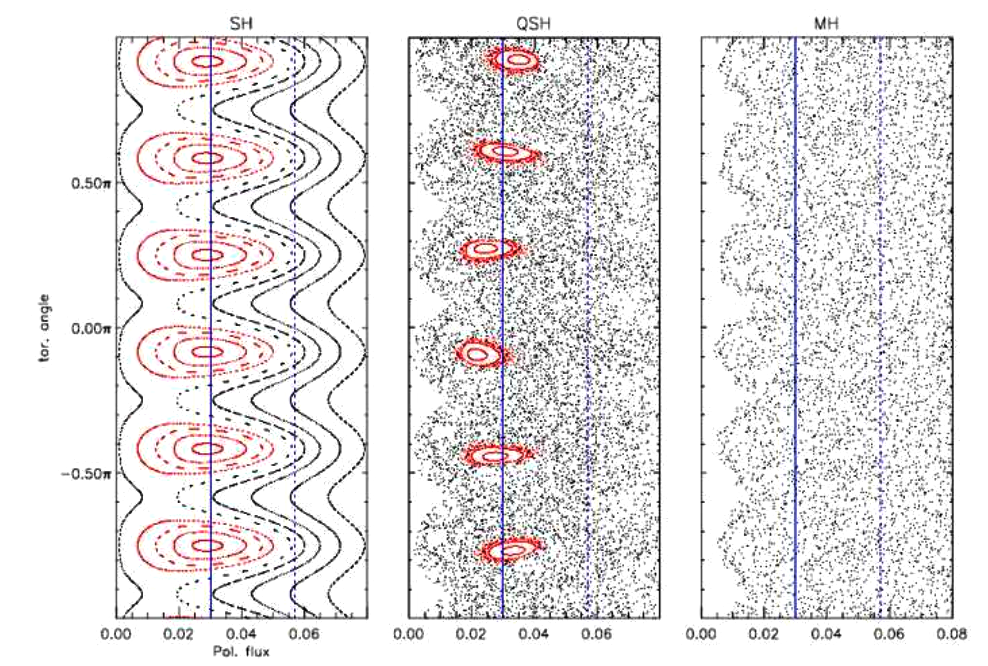
\includegraphics[height=4.2cm]{img/2_eq/poincare_QSH.png} \label{img:MHQSH_a}}
    \subfigure[]{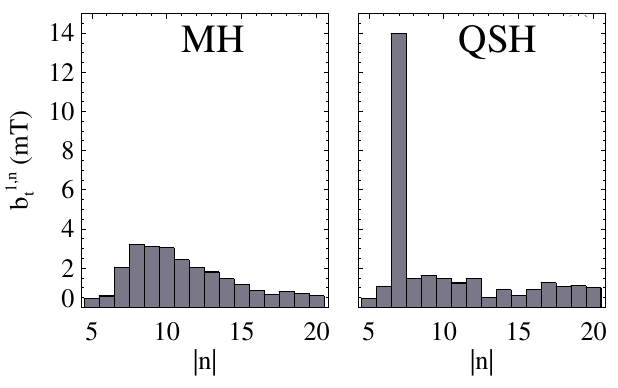
\includegraphics[height=4cm]{img/2_eq/QSH_modes_example.png} \label{img:MHQSH_b}}
    \caption{Poincaré plots of the magnetic configuration mad with ORBIT code (a) with SH, QSH, MH magnetic mode configuration     respectively; an example of toroidal mode number spectra m = 1, n modes in a VS (Virtual Shell controlled) RFX-mod discharge (b). }
    \label{img:MHQSH_b}
\end{figure}















%  ____  _______  __                         _ ____  
% |  _ \|  ___\ \/ /     _ __ ___   ___   __| |___ \ 
% | |_) | |_   \  /_____| '_ ` _ \ / _ \ / _` | __) |
% |  _ <|  _|  /  \_____| | | | | | (_) | (_| |/ __/ 
% |_| \_\_|   /_/\_\    |_| |_| |_|\___/ \__,_|_____|

\section{RFX-mod2 \\ \small{a chance for a better controllable machine}}
\cite{SONATO2003161}
\cite{doi:10.1063/1.4806765}
\cite{martin_RFX_overview}

% CHALLENGES AND SOLUTIONS IN THE DESIGN OF RFX-MOD2, A MULTI CONFIGURATION MAGNETIC CONFINEMENT EXPERIMENTAL DEVICE

% RWR
RFX-mod is a flexible \ac{RFP} toroidal device (major radius $R=2 m$ and minor radius $a=0.46 m$) with plasma current up to 2 MA and volume $10 m^3$ \cite{SONATO200597}. As in all RFPs, plasma heating is purely ohmic; \acl{RFP} could in principle obtain fusion power with ohmic heating only, and with a magnetic field much smaller than in a tokamak—avoiding superconducting coils. RFX-mod is equipped with a very powerful system of active coils for feedback control of plasma MHD stability: 192 coils, independently driven, cover the whole plasma surface.


\section{RFX diagnostics}
% kind of RFX diagnostics
In fusion machines the number of signals to be acquired is very high, they can be classified by the nature of the diagnostics:
signals from magnetic probes, from Soft X-Ray detectors, form probes derived from photodiodes, from Langmuir probes, etc.
%
We can further divide the diagnostics into 3 main families:
\begin{itemize}
    \item Magnetics, and the related plasma current, loop potentials, etc.
    \item Spectroscopic diagnostics, like XUV-VUV or X-Ray, or electron cyclotron emission. 
    \item Reflectometers and interferometers, which manipulate optical and laser signals by performing demodulation.    
          Measurement of electron temperature Te provided by Thomson scattering of laser light (TS)
\end{itemize}


%
\begin{figure}[ht!]
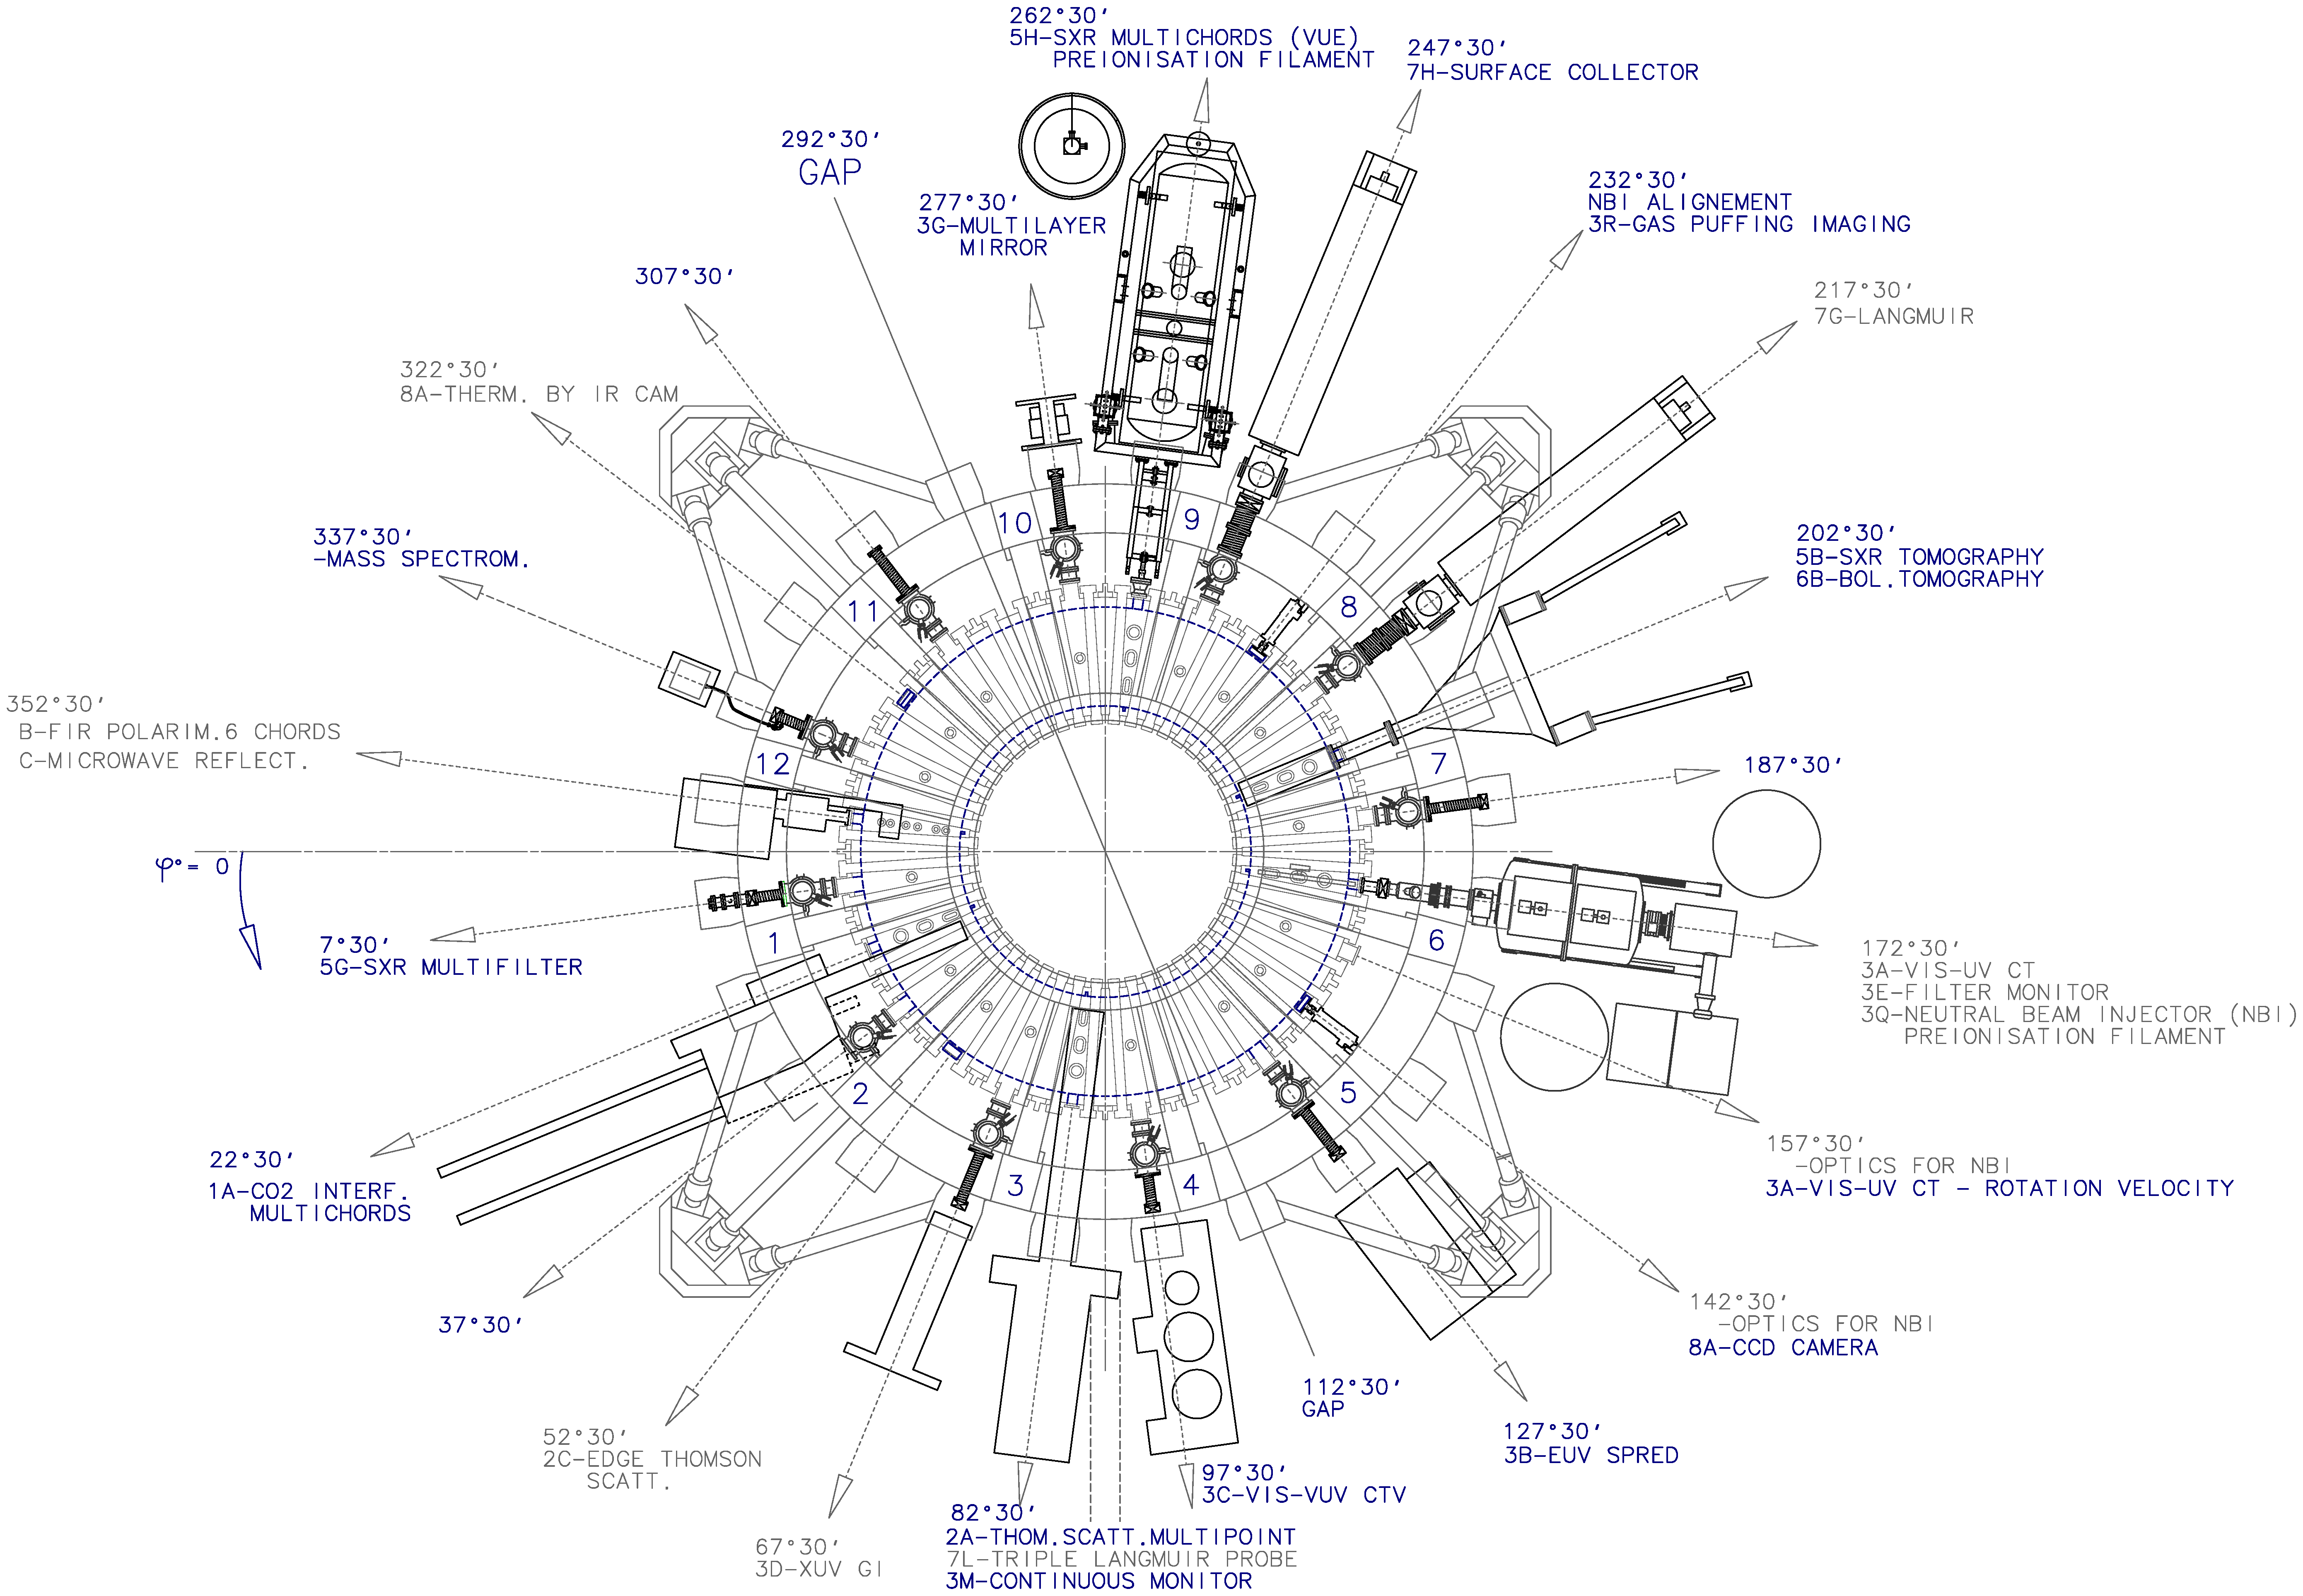
\includegraphics[width=1\textwidth]{img/rfx/Layout_Diagnosiche_AA10005.eps} \centering
% TODO: add figures
\caption{RFX map of diagnostics with related toroidal position.}
\label{rfx}
\end{figure}
%

\subsection{Thomson Scattering}
The Thomson scattering  has been a key-factor diagnostic at RFX since the initial operations for the study of RFP plasma configuration, yielding a fundamental correlation between the electron temperature diffusivity and the magnetic fluctuations that link the plasma confinement to the dynamo related modes~\cite{}. This also evolved in the possibility to identify a hot asymmetric island when the temperature gradient extends to the plasma core in the \ac{QSH} state.
During the first operation of RFX the diagnostic was composed by a single pulse of laser from ruby diode ( $\lambda = 694 nm$ ) passing through the plasma in the equatorial plane, and two grating photo-multipliers spectrometers.
This apparatus presented some limitations: from the precision point of view it suffered of a poor quantum efficiency of the multialkali cathode of the photo-multiplier (MCP-PMT) resulting in a general lack of sensitivity and noisy profile at low electron temperatures. On the other hand the 20 chords acquisition that characterized the acquired profile with a 24 mm spatial resolution was unable to effectively investigate the details of the QSH magnetic islands.

Since the 2005 with the experiment upgrade to RFX-mod the diagnostic was completely renewed. In particular the replacement of the grating spectrometers with a set of four filter polycromators with avalanche photo-diodes (APD) provided a 30 times higher sensitivity and 84 points profile with a new narrow grained 7mm resolution ( $r/a$ from -0.96 to 0.84 ).
The new Nd:YLF laser diode ($\lambda=1053 nm$) located 15 m away from the center of the vacuum vessel, can produce an up to 7 J burst of 10 pulses per experiment shot. with a single light emission duration of 20ns FWHM (full-width at half maximum).

The light passing through plasma on the equatorial plane scatter in all directions and is collected by photo-multipliers at three different windows at the end of short vertical ports. The 84 pairs of quartz fibers look at all the plasma poloidal angles by magnifying optics located at the ports. All fibers can be also moved by a special mechanical support that can self orient during the experiment setup state; at the same time all optics can also automatically adjust focus to the desired radial position of interest.
A further side by side light path decomposes the acquired spectrum in 4 channels using a series of relay lenses.
%
The small amount of the solid angle covered by the acquisition, together with all this set of filters applied both at the input beam - aiming at reducing the stray light and maintaining the focus -, and at the output - for the selection of the plasma region of interest and for the decomposition of the energy spectrum - are the main reason for the required high power input.
%
This leads to a scattered set of acquisition pulses that are not continuously reconstructing the overall shape of plasma temperature but they are reduced to a small set of usually 10 time events per pulse.
%
The recording system is also quite complex: for RFX-mod the detected signal has been acquired by a modular 4-channels cPCI board dedicated for each of the spectrometers, acquiring data at 500 Msps each.

\subsection{Soft X Ray}

% We chose the most reliable and fast response diagnostics ... (SXR and Magnetic coils MHD)
% Other possible diagnostics can be added ( cope with time dim )
% Possibility to trigger in realtime other diagnostics ( i.e. Thomson Scattering )

In 1996 a SXR tomographic system was installed in a RFP (Reversed Field
Pinch) experiment for the first time \cite{Franz_2001}. 
As shown in the previous sections the RFP configuration is keen to produce a large amount of magnetic instabilities due to the low profile of the safety factor. The current driven instabilities that are very common in RFPs can grow in the core of plasma producing the so called ``magnetic islands''. 
At the islands toroidal positions the SXR emits more, and localized regions are identified. 
Imaging of these SXR structures was allowed by the application of the Fourier-Bessel expansion of the Cormack inversion, as proposed by Nagayama in~\cite{Bonomo25}. 
The algorithm is studied to achieve a good image reconstruction even with few harmonics, as the case of SXR where the acceptance of integral measuring cords  is affected by the small (and few) openings in the vessel. If the amplitude of the many magnetic instabilities is approximately the same, as in the case of the so-called \acl{MH}, the reconstructed SXR emissivity is almost symmetric; it is shown in~\Figure{\ref{fig:MH_QSH_example}a}. Conversely, in presence of an instability where a single mode dominates, a magnetic island is sustained and, as shown in~\Figure{\ref{fig:MH_QSH_example}b}, an asymmetric emissivity profile with a localized bight region is detected. This state is called \acl{QSH}.
%
\begin{figure}
    \centering
    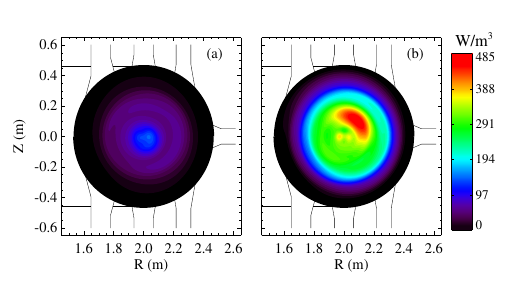
\includegraphics[height=5cm]{img/2_eq/MH_QSH_example.png}
    \caption{Contour plot of the reconstructed SXR emissivity for a standard multiple helicity (MH) configuration (a), and for a quasi-single helicity (QSH) configuration (b); acquired at RFX by SXR3 device; the color bar is in W /m3 .
    }
    \label{fig:MH_QSH_example}
\end{figure}
%
In the currently operating RFP experiments, and in RFX-mod likewise, the time evolution of such instabilities is of the order of few ms. This sets a requirement on the bandwidth of the measurements up to several hundreds of kHz.

A new SXR diagnostic named DSX3 have been installed in one of the equatorial ports of RFX-mod chamber; it completes the existing tomographic diagnostic maintaining several primary characteristics of the original SXR manipulators. Further
features have been added: a larger number of acquired cords, a wider flexibility in the detection system geometry and the possibility of dynamically selecting different ranges of detected radiation energy.
%
\begin{figure}
    \centering
    \subfigure[]{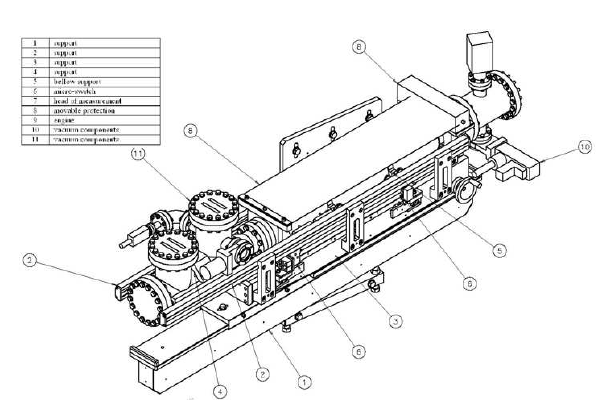
\includegraphics[height=5cm]{img/rfx/SXR_sketch.png}}
    \subfigure[]{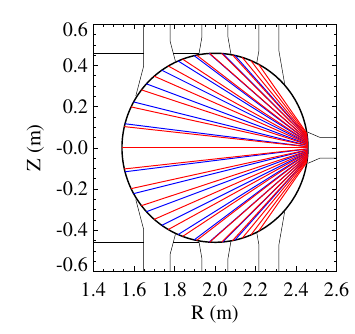
\includegraphics[height=5cm]{img/rfx/SXR3_cords.png}}
    \caption{DXS3 perspective view (a), and the geometry of the lines of sight of DSX3 (at the tomography toroidal section
             of RFX-mod vessel) for the three rows of photodiodes (b): the red lines correspond to the
             27 diodes of the central row, while the chords for the two external rows (blue lines) are perfectly
             overlapping }
    \label{fig:DSX3_sketch}
\end{figure}




% \section{The complete “SCHEMA” from sensors to plasma parameters}
